\subsection{Web Content Management}

\subsubsection{Overview}

What is Web Content Management (WCM)?  The essence of WCM is that it
allows non-technical people to rapidly edit content on a web site.
Traditionally, a web site needs highly skilled HTML web \emph{masters} to
update the web site.  However, these web master, after they have built
the web site, tend to move on to building other web sites.  Without
these people available to keep the web site relevant, the web site
information tends to become stale and out dated.
  
WCM seeks to address this problem.  It allows web masters to build a
WCM site that can be \emph{maintained} by non-technical users on an
ongoing basis.  This is achieved by providing the non-technical users
familiar WYSIWIG (What You See Is What You Get) editors that look much
like familiar word-processing tools.
  
\begin{figure}[h!]
  \centering
  \fbox{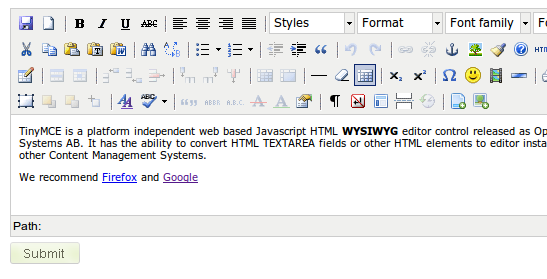
\includegraphics[width=130mm]{images/wysiwigHtmlEditor}}
  \caption{WYSIWYG Editor}
\end{figure}

\subsubsection{How does this work in practice?}

In a day to day usage scenario, a business user would decide he wanted
to change some content on a web page.  They would navigate to that
page and press a special set of keys and the web page then displays
little pencil icons everywhere the user is allowed to modify content.
They simply click the pencil icon and then they are presented with the
\emph{WYSIWIG} like the one shown above, and then they can edit the
content.  Once they save the section of the web page they edited, the
content is either automatically updated on the production site, or
alternatively it may be subjected to a workflow approval process.
	
\subsubsection{The changed role of the Web Master}
Obviously for all this `magic' to occur, there needs to be something
in-place other than plain old static HTML content. The basic
architecture is that 90\% of the system is contained within the Oracle
Universal Content Management (UCM) system.  Additionally you place a
Web Server in front of UCM to send the HTML the UCM system generates
to the client browser.  The following diagram lays out the basic
architecture of an Oracle WCM site.
	
\begin{figure}[h!]
  \centering
  \fbox{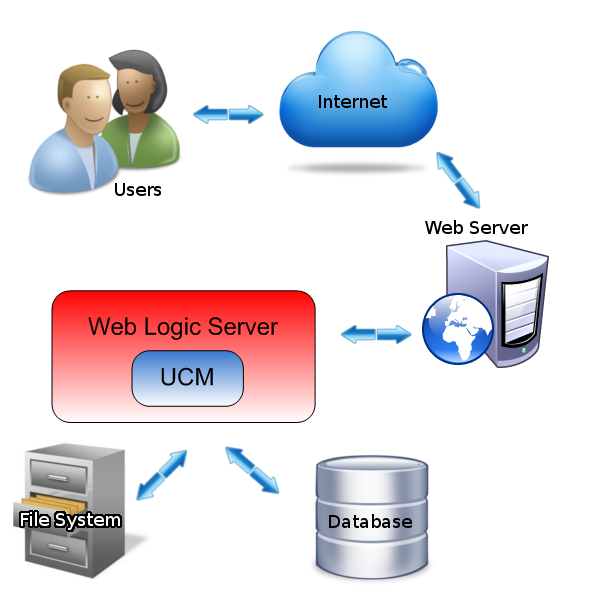
\includegraphics[width=130mm]{images/basicUcmArchitecture}}
  \caption{UCM Basic Architecture}
\end{figure}

\clearpage

Now the web master creates special `Site Studio' web sites, using the
tools provided by Oracle WCM, and finally we have a WebContent
Management website, versus some other type of web site.

\subsubsection{A new business administrator role introduced}
Along with the core web master who develops the basic framework for
your site, there is another sudo-administrator role introduced with
web content management.  This user requires technical skills somewhere
between the Web Master and the end Business user.  This user is given
the following additional privileges:

\begin{itemize}
\item Create new sections for the website
\item Rearrange the navigation for a website
\end{itemize}

So in summary there are three distinct roles when working with WCM
sites.  The number of users in that role and the technical level of
difficulty are depicted in the following image:

\begin{figure}[h!]
  \centering
  \fbox{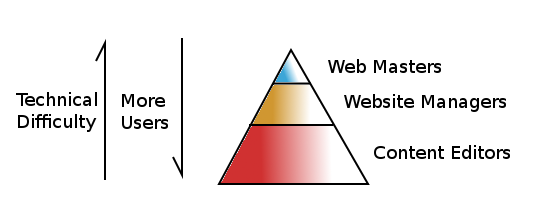
\includegraphics[width=130mm]{images/wcmRoles}}
  \caption{WCM Roles}
\end{figure}
\clearpage